%%%%%%%%%%%%%%%%%%%%%%%%%%%%%%%%%%%%%%%%%%%%%%%%%%%%%%%%%%%%%%%%%%%%%%%%%%%%%%%%%%%%%%%%%
% 
% Document class for MEEC@DEE@ISEP dissertations, by Vitor M. R. Cunha - v1.3, Jul 2021
% Suggestions and comments are welcomed (vrc at isep dot ipp dot pt).
%
% Template provided as is, NO SUPPORT will be given.
% NO questions related to LaTeX will be answered, go to
% https://ftp.eq.uc.pt/software/TeX/info/lshort/english/lshort.pdf, or search the web.
%
% The DEE document class uses the LaTeX book base class, the original work credits are
% in the document class file.
%
% Overleaf template direct link:
% https://www.overleaf.com/latex/templates/isep-meec-msc-thesis-slash-dissertation-latex-template/zdyypsqypqnm
% or go to https://www.overleaf.com/gallery/, and search for: ISEP MEEC
%
%%%%%%%%%%%%%%%%%%%%%%%%%%%%%%%%%% MAIN SETTINGS %%%%%%%%%%%%%%%%%%%%%%%%%%%%%%%%%%%%%%%%

\documentclass[
MEECAS,			% Use this option to select your DEE degree, options: MEECAS, MEECSA, MEECPI, MEECTE
portuguese,		% Select document language, options: portuguese or english
%draft,			% Uncomment for draft mode (no pictures, no links, overfull hboxes) 
]{DEEclass}

% Use the 'preamble.tex' file (root folder) do add packages and macros. Keep your main.tex file clean.

% FYI, the following packages are preloaded with the document class:
% longtable, xcolor, graphicx, booktabs, caption, csquotes, hyperref,
% calc, listings, datetime2, siunitx, geometry, enumitem

%%%%%%%%%%%%%%%%%%%%%%%%%%%%%%%%%%%%%%%%%%%%%%%%%%%%%%%%%% extra packages
\usepackage{amsmath}		% the main package in the AMS-LATEX distribution
\usepackage{amsfonts}		% extended set of fonts for use in mathematics
\usepackage{amssymb}		% adds new symbols to be used in math mode
\usepackage{mathrsfs}		% math fonts, e.g., Laplace
\usepackage{float}			% provides the H float modifier option
\usepackage{multirow}		% tables \multirow command
\usepackage{subcaption}		% enables subfigures
\usepackage{lscape}			% for landscape mode
\usepackage{verbatim}		% new verbatim environment, \begin{comment}...\end{comment}, \verbatiminput
%\usepackage{pgfgantt}		% for Gantt charts, see https://ctan.org/pkg/pgfgantt
%\usepakage{siunitx}%valores c/unidades SI
\usepackage{eurosym}
%add extra packages if needed here
% Please add the following required packages to your document preamble for table:
 \usepackage[table,xcdraw]{xcolor}
% Beamer presentation requires \usepackage{colortbl} instead of \usepackage[table,xcdraw]{xcolor}


\sisetup{
	per-mode = symbol,
	output-decimal-marker = {,}
}
\DeclareSIUnit{\eurocurrency}{\text{\euro}}
%%%%%%%%%%%%%%%%%%%%%%%%%%%%%%%%%%%%%%%%%%%%%%%%%%%%%%%%%% temp packages
\usepackage{lipsum}						% for fake text
%\usepackage[textsize=tiny]{todonotes}   % enable To-do notes, use the option "disable" to hide all notes, usage \todo{}

%\usepackage{draftwatermark}			% prints a watermark overlay, uncomment if needed
%\SetWatermarkText{**DRAFT**}
%\SetWatermarkScale{1}
%\SetWatermarkColor[gray]{0.8}

%%%%%%%%%%%%%%%%%%%%%%%%%%%%%%%%%%%%%%%%%%%%%%%%%%%%%%%%%% settings
\AtBeginDocument{					% Rendered PDF metadata:
\hypersetup{pdftitle=\ttitle} 	    % Sets the PDF title to your dissertation title
\hypersetup{pdfauthor=\authorname} 	% Sets the PDF author to your name
}

%%%%%%%%%%%%%%%%%%%%%%%%%%%%%%%%%%%%%%%%%%%%%%%%%%%%%%%%%% user macros

%....








		 
\makeglossaries
%%%%%%%%%%%%%%%%%%%%%%%%%%%%% DISSERTATION INFORMATION %%%%%%%%%%%%%%%%%%%%%%%%%%%%%%%%%%

\thesistitle{JavaFX} % Your dissertation title

\subdate{Novembro, 2026} % Uncomment for a static submission date, or leave it as a comment for automatic date 

\author{Eduardo Miguel Moreira Junqueira}	% Your name
\studentnumber{1251561}	% Your student number
\studentemail{1251561@isep.ipp.pt}	% Your student email address  

\advisor{Benedita Malheiro}{mbm@isep.ipp.pt}	% Your advisor's name and email
%\coadvisor{Nome do Coorientador}{xxx@isep.ipp.pt}	% Your co-advisor's name and email, comment this line if not needed
%\company{Nome da Empresa, Lda.}	% The company name where you developed your work, comment this line if not needed
%\supervisor{Nome do Orientador da Empresa}{xxx@emailaddress.com}	% Your supervisor's name, comment this line if not needed

%%%%%%%%%%%%%%%%%%%%%%%%%%%%% USER DEFINED LISTS %%%%%%%%%%%%%%%%%%%%%%%%%%%%%%%%%%%%%%%%
%----------------------------------------------------------------------------------------
%	ACRONYMS LIST
%----------------------------------------------------------------------------------------

% Only the used entries will be displayed in the printed list, ie, you need to used a acronym at least once
% Full name in italic if not in the main document language

%acronym definition usage:
%\newacronym{<tag>}{<acronym>}{<full name>}

\newacronym{wys}{WYSIWYG}{\textit{What You See Is What You Get}}
\newacronym{dee}{DEE}{Departamento de Engenharia Electrotécnica}
\newacronym{api}{API}{\textit{Application Programming Interface}}
\newacronym{ascii}{ASCII}{\textit{American Standard Code for Information Interchange}}
\newacronym{html}{HTML}{\textit{HyperText Markup Language}}
\newacronym{isep}{ISEP}{Instituto Superior de Engenharia do Porto}
\newacronym{meec}{MEEC}{Mestrado em Engenharia Electrotécnica e Computadores}
\newacronym{usb}{USB}{\textit{Universal Serial Bus}}
\newacronym{pdf}{PDF}{\textit{Portable Document Format}}
\newacronym{uc}{UC}{\textit{Unidade Curricular}}
\newacronym{rinte}{RINTE}{\textit{Redes Inteligentes e Serviços}}
\newacronym{www}{WWW}{\textit{World Wide Web}}
\newacronym{http}{HTTP}{\textit{Hypertext Transfer Protocol}}
\newacronym{jdk}{JDK}{\textit{Java Development Kit}}

% Acronyms introduced in Chapters 2 to 5 (Problema, Solução, Testes e Avaliação, Conclusões)
\newacronym{rest}{REST}{\textit{Representational State Transfer}}
\newacronym{json}{JSON}{\textit{JavaScript Object Notation}}
\newacronym{sql}{SQL}{\textit{Structured Query Language}}
\newacronym{jdbc}{JDBC}{\textit{Java Database Connectivity}}
\newacronym{sgbd}{SGBD}{Sistema de Gestão de Base de Dados}
\newacronym{ide}{IDE}{\textit{Integrated Development Environment}}
\newacronym{crud}{CRUD}{\textit{Create, Read, Update, Delete}}
\newacronym{dao}{DAO}{\textit{Data Access Object}}
\newacronym{fk}{FK}{\textit{Foreign Key}}
			% Edit to define your acronyms entries list

%%%%%%%%%%%%%%%%%%%%%%%%%%%%%%%%%%%%%%%%%%%%%%%%%%%%%%%%%%%%%%%%%%%%%%%%%%%%%%%%%%%%%%%%%
\begin{document}
\frontmatter

%----------------------------------------------------------------------------------------
%	TITLE PAGES
%----------------------------------------------------------------------------------------
\pagestyle{plain} % Default to the plain heading style until the thesis style is called for the body content
\printcoverpage
\printaftercoverpage
\cleardoublepage















%%%%%%%%%%%%%%%%%%%%%%%%%%%%%%%%%%% FRONTMATTER %%%%%%%%%%%%%%%%%%%%%%%%%%%%%%%%%%%%%%%%%
% Consider the following front matter sections provided as separate files in the 'front' folder.
% Comment the lines regarding the sections you will not use, or edit the file contents as needed

%%----------------------------------------------------------------------------------------
%	DEDICATION
%----------------------------------------------------------------------------------------

\dedicatory{
(Opcional) Poderá usar esta secção para dedicar o trabalho a alguém\ldots
} 
		% Edit if you want to dedicate your work to someone, or comment this line if not used
%%----------------------------------------------------------------------------------------
%	ACKNOWLEDGEMENTS
%----------------------------------------------------------------------------------------

\begin{acknowledgements}

(Opcional) Agradecimentos que sejam devidos\ldots

\end{acknowledgements}
	% Edit to add the due acknowledgements, or comment this line if not used
%----------------------------------------------------------------------------------------
%	ABSTRACT PAGES
%----------------------------------------------------------------------------------------

% IMPORTANT NOTE: the abstract must always be written in two languages. If the dissertation
% is written in Portuguese you have selected 'portuguese' as the language in the document class.
% Therefore, the portuguese version of the abstract must come first, so write it in the
% below area denoted by 'MAIN LANGUAGE ABSTRACT'. The english version follows in the
% 'SECOND LANGUAGE ABSTRACT' section.
% If the dissertation is written in English, first will come the abstract in English
% ('MAIN LANGUAGE ABSTRACT') and then in Portuguese ('SECOND LANGUAGE ABSTRACT').

\begin{abstract}
%%%%%%%%%%%%%%%%%%%%%%%%%%%%%% MAIN LANGUAGE ABSTRACT %%%%%%%%%%%%%%%%%%%%%%%%%%%%%%%%%%
A \textit{framework JavaFX}, será estudada e implementada neste relatório técnico-científico, com a criação de uma aplicação distribuída esta tecnologia será apresentada.



Aqui deverá ser apresentado o resumo de todo o trabalho efetuado. Esta secção não deverá exceder uma página.

Deve contextualizar o problema que pretende resolver ou a hipótese que irá formular, procure evidenciar as vantagens e desvantagens (se as houver) da solução encontrada, como também a forma através da qual a solução/hipótese foi validada. Neste último ponto, deverá referir-se aos desenvolvimentos efetuados, e à forma como validou (conformidade) e avaliou (desempenho) a solução encontrada.

A dissertação deve conter sempre duas versões do resumo: uma primeira no idioma do texto principal e a segunda num outro idioma. Este \textit{template} assume que os dois idiomas em consideração são sempre Português e Inglês, assim, a classe irá colocar os cabeçalhos respetivos de acordo com o idioma selecionado nas opções da classe no ficheiro \file{main.tex}. 

%----------------------------------------------------------------------------------------

\vspace*{10mm} 
\noindent
\textbf{\keywordslabel}: \textit{JavaFX}, Lista, separada por vírgulas, de palavras, frases, ou acrónimos chave no âmbito do trabalho descrito neste texto. 

%%%%%%%%%%%%%%%%%%%%%%%%% END OF THE MAIN LANGUAGE ABSTRACT %%%%%%%%%%%%%%%%%%%%%%%%%%%%%%
\end{abstract}
\begin{secondlangabstract}
%%%%%%%%%%%%%%%%%%%%%%%%%%%%%% SECOND LANGUAGE ABSTRACT %%%%%%%%%%%%%%%%%%%%%%%%%%%%%%%%%%
The framework JavaFX, will be studied and implemented in this theoretical-cientific paper, with the creation of distributed aplication, this tecnology will be presented.


%----------------------------------------------------------------------------------------

\vspace*{10mm} 
\noindent
\textbf{\keywordslabel}: JavaFX,

%%%%%%%%%%%%%%%%%%%%%%%%%% END OF THE SECOND LANGUAGE ABSTRACT %%%%%%%%%%%%%%%%%%%%%%%%%%%%%
\end{secondlangabstract}

			% Edit the file to write the dissertation Abstract. Two languages are always required.
%----------------------------------------------------------------------------------------
%	FONTMATTER LISTS
%----------------------------------------------------------------------------------------
\pdfbookmark[0]{\contentsname}{toc}
\tableofcontents 	
\glsresetall
%----------------------------------------------------------------------------------------

% Of the following lists, comment the ones you will not use in your document

\listoffigures 			% Prints the list of figures

\listoftables 			% Prints the list of tables

%\printlistoflistings	% Prints the list of listings (source code segments)

\printlistofterms		% Prints the list of USED terms (glossary)

\printlistofacronyms{XXXXXXXXI} % Prints the list of USED acronyms
% Change the argument with random letters to adjust the left alignment of the acronyms full name column

\printlistofsymbols		% Prints the list of ALL defined symbols
	% Edit the file to select the lists to be shown (figures, tables, source code segments, glossary, acronyms, symbols)

%%%%%%%%%%%%%%%%%%%%%%%%%%%%%%%%%%% MAINMATTER %%%%%%%%%%%%%%%%%%%%%%%%%%%%%%%%%%%%%%%%%
\mainmatter 
\pagestyle{thesis} 				

% Include the chapters of the dissertation as separate files from the 'chapters' folder

\begin{comment}

Resumo
Abstract
Glossário
Introdução
	Contextualização
	Objetivos
	Planeamento
	Organização do Documento
Problema
	Definição
	Requisitos
		Funcionais (Atores, Caso de Uso)
		Técnicos (Latência, carga, etc.)
	Sumário
Solução (Conceção e Implementação)
	Ferramentas e Tecnologias
	Arquitetura
	Modelo de Dados
	Front-end
	Back-end
	Sumário
Testes e Avaliação
	Funcionais
	Desempenho (volume de dados e latência por caso de uso e impacto da carga no caso maior latência)
	Usabilidade
	Discussão 
	Sumário
Conclusão
	Sumário dos Resultados
	Limitações
	Desenvolvimento Futuro	
Bibliografia

Aula 21/10/2026 prática de RINTE dados:
\begin{itemize}

\item procurar sempre em: https://ctan.org/pkg/siunitx 
\item no caso de siunitx https://ftp.eq.uc.pt/software/TeX/macros/latex/contrib/siunitx/siunitx.pdf 
\item Escrever sempre em 3 pessoa.
\item Frases Ativas.
\item Figuras no inicío ou fim da página não no final em anexos.
\item Escrever sempre em itálicos tudo o que não está no dicionário com exceção de nomes próprios de empresas ou produtos .
\end{itemize}
\unit{\kilogram\metre\per\second}

\SI{156000}{\eurocurrency}
\SI{150000}{\milli\gram}

\end{comment}
%%%%%%%%%%%%%%%%%%%%%%%%%%%%%%%%%%%% Chapter INTRODUÇÃO

\chapter{Introdução} 	% Main chapter title
\label{Chapter1} 		% For referencing the chapter elsewhere, usage \ref{Chapter1}

A este capítulo introdutório  a contextualização e organização do documento descrevem o relatório de uma forma geral, enquanto que os objetivos e o planeamento demonstram mais ao pormenor o estudo e a análise que foi  feito ao longo deste relatório.

%%%%%%%%%%%%%%%%%%%%%%%%%%%%%%%%%%%% Contextualização

\section{Contextualização}
\label{sec:Ch1.1}

\noindent No âmbito da \ac{uc} de \ac{rinte},  será realizado o trabalho nº1, sobre uma tecnologia de suporte ao desenvolvimento de aplicações.~A elaboração deste  relatório técnico-científico é sobre a tecnologia \textit{JavaFX Framework}.~A entrega deste relatório será acompanhada também por código e apresentação exclusivamente para esta \ac{uc} de \ac{rinte} da autoria própria do aluno, que realizou o trabalho, Eduardo Miguel Moreira Junqueira.

\noindent \textit{JavaFX}, uma plataforma de software criada por Sun Microsystems em 2008. Em 2011 tornou-se \textit{open-source} e no ano seguinte migrou para Oracle Corporation's \ac{jdk}. Em 2018 Oracle Corporation's, decidiu não agregar mais esta tecnologia e então formou-se a comunidade representante atualmente com a parceria da GLUON, nomeada de \textit{OpenJFX}\cite{Pereira2020},\cite{OpenJFX}.%JavaFX. (n.d.). Community OpenJFX. Retrieved October 29, 2026, from https://openjfx.io/



%%%%%%%%%%%%%%%%%%%%%%%%%%%%%%%%%%%% Objetivos

\section{Objetivos}
\label{sec:Ch1.2}
 %apresentar de forma clara os objetivos que se propõe atingir
\noindent O objetivo principal deste trabalho prático é estudar e  implementar a tecnologia \textit{JavaFX Framework} de suporte ao desenvolvimento de aplicações distribuídas.

\noindent Esta aplicação distribuída, que será criada como exemplo demonstrativo da tecnologia em estudo, tem como âmbito seguir uma arquitetura de três camadas, ou seja, \textbf{I-} cliente gráfico em \textit{JavaFX},  \textbf{II-} servidor em \textit{Tomcat},  \textbf{III-} base de dados em \textit{MySQL}.

\noindent Inicialmente será realizado um teste de implementação em conjunto com a pesquisa, para verificar a tecnologia a funcionar com as devidas bibliotecas necessárias.

\noindent De seguida, será implementado um projeto nomeado "Gestão de Tarefas",~com dois tipos de clientes, o administrador e o utilizador.

\begin {enumerate}
\item Administrador:~usa métodos \ac{http} do tipo \textit{GET,POST,PUT,DELETE}  para controlar todas as tarefas.
Também usa métodos \ac{http} do tipo \textit{GET,POST,DELETE} para controlar todos os utilizadores.
\item Utilizador:~usa métodos \ac{http} do tipo \textit{GET,POST,PUT}  para controlar apenas as suas tarefas.
\end {enumerate}
%%%%%%%%%%%%%%%%%%%%%%%%%%%%%%%%%%%% Planeamento

\section{Planeamento}
\label{sec:Ch1.3}

A tabela seguinte \ref{tab:cronograma}, demonstra as principais tarefas que foram realizadas de forma autónoma, ao longo de 5 semanas, após a atribuição da tecnologia em estudo.
% Cores próximas das usadas no Excel
\definecolor{fundo}{HTML}{C9C9C9}
\definecolor{pesquisa}{HTML}{AA55A0}
\definecolor{relatorio}{HTML}{32A34A}
\definecolor{implementacao}{HTML}{1084A7}
\definecolor{validacao}{HTML}{B75A28}

% Célula ativa: recebe uma cor e apresenta o valor 1
\newcommand{\ativo}[1]{\cellcolor{#1}1}


\begin{table}[htbp]
    \centering
    \renewcommand{\arraystretch}{1.5}
    \setlength{\tabcolsep}{8pt}

\begin{tabular}{|>{\columncolor{fundo}}l|*{5}{>{\columncolor{fundo}}c|}}
        \hline
        Tarefas
        & 28/9 a 4/10
        & 5/10 a 11/10
        & 12/10 a 18/10
        & 19/10 a 25/10
        & 26/10 a 1/11 \\
        \hline

        Pesquisa
        & \ativo{pesquisa}
        & \ativo{pesquisa}
        & \ativo{pesquisa}
        & \ativo{pesquisa}
        & \ativo{pesquisa} \\
        \hline

        Relatório
        & 0
        & 0
        & 0
        & \ativo{relatorio}
        & \ativo{relatorio} \\
        \hline

        Implementação
        & 0
        & 0
        & \ativo{implementacao}
        & \ativo{implementacao}
        & \ativo{implementacao} \\
        \hline

        Validação
        & 0
        & 0
        & 0
        & 0
        & \ativo{validacao} \\
        \hline
    \end{tabular}

    \caption{Cronograma das tarefas.}
    \label{tab:cronograma}
\end{table}


%%%%%%%%%%%%%%%%%%%%%%%%%%%%%%%%%%%% SECTION 5

\section{Organização do Documento}
\label{sec:Ch1.4}

\noindent Nos seguintes capítulos, o problema contém a definição e os requisitos quer funcionais, quer técnicos. A solução explicita as ferramentas e tecnologias utilizadas, identificando a arquitetura, os modelo de dados, \textit{front-end, back-end}. Os testes e avaliação demonstram as funcionais o desempenho e também a usabilidade. A conclusão retrata o sumário dos resultados com as devidas limitações e o desenvolvimento futuro do trabalho nº2.	




%Introdução
% Chapter 2

\chapter{Problema}	%The main chapter title
%\chaptermark{O \textit{Template}}	%Short version for page header. Comment if not needed
\label{Chapter2}	%For referencing the chapter elsewhere, use \ref{Chapter2} 


\noindent O projeto  de gestão de tarefas pretende demonstrar a tecnologia numa arquitetura distribuída de três camadas. Neste capítulo é apresentada a definição do problema, os requisitos funcionais e técnicos da solução.
%%%%%%%%%%%%%%%%%%%%%%%%%%%%%%%%%%%% Section :Definição

\section{Definição}
\label{sec:Ch2.1}

\noindent No contexto académico, o projeto de gestão de tarefas  é um exemplo criado com o intuito de explicar a tecnologia em estudo. ~O problema surge assim em dois campos distintos:
\begin {itemize}
\item Validação de solução gráfica da tecnologia em estudo.
\item Integração do servidor  \textit{Tomcat} para comunicar com a base de dados  \textit{MySQL} para o serviço remoto da aplicação distribuída.
\end {itemize}

\noindent A solução proposta tem como intuito, validar os conceitos lecionados na \ac{uc} de \ac{rinte}, nomeadamente a comunicação entre um cliente e um servidor através de um serviço \textit{web} baseado no protocolo \ac{http} de três camadas.


\section{Requisitos}
\label{sec:Ch2.2}

\noindent Os requisitos da aplicação Gestão de Tarefas dividem-se em requisitos funcionais, que descrevem o comportamento esperado do sistema do ponto de vista dos seus utilizadores, e requisitos técnicos, que definem as regras não funcionais que a solução deve respeitar.

\subsection{Funcionais}


\noindent A aplicação distribuída tem dois tipos de atores, com níveis de permissão distintos:

\begin{itemize}
	\item \textbf{Administrador} -- responsável pela gestão de todas as tarefas do sistema e pela gestão dos utilizadores registados;
	\item \textbf{Utilizador} -- responsável apenas pela gestão das tarefas que lhe foram atribuídas ou que criou.
\end{itemize}

\noindent A Tabela~\ref{tab:usecases} resume os principais casos de uso identificados, associando-os ao ator responsável e ao método \ac{http} que a interface \ac{rest} do \textit{back-end} segue neste projeto.

\begin{table}[htb]
	\caption{Casos de uso e correspondência com os métodos \ac{http} da \ac{api}.}
	\label{tab:usecases}
	\centering
	\begin{tabular}{l l c}
	\toprule
	\tabhead{Ator} & \tabhead{Caso de Uso} & \tabhead{Método \ac{http}} \\
	\midrule
		Administrador \& Utilizador & Autenticar-se no sistema & \code{POST} \\
		Administrador & Criar tarefa & \code{POST} \\
		Administrador & Consultar todas as tarefas & \code{GET} \\
		Administrador & Atualizar qualquer tarefa & \code{PUT} \\
		Administrador & Eliminar qualquer tarefa & \code{DELETE} \\
		Administrador & Criar utilizador & \code{POST} \\
		Administrador & Consultar utilizadores & \code{GET} \\
		Administrador & Eliminar utilizador & \code{DELETE} \\
		\midrule
		Utilizador & Criar tarefa própria & \code{POST} \\
		Utilizador & Consultar as suas tarefas & \code{GET} \\
		Utilizador & Atualizar tarefa própria & \code{PUT} \\
	\bottomrule
	\end{tabular}
\end{table}

\subsection{Técnicos}

\noindent Para além dos requisitos funcionais, a solução deve ainda respeitar os seguintes requisitos técnicos:

\begin{itemize}
	\item \textbf{Autenticação e autorização} -- o acesso à \ac{api} deve ser condicionado à autenticação do utilizador, devendo o \textit{back-end} validar, em cada pedido, se o ator autenticado possui permissões para a operação solicitada;
	\item \textbf{Portabilidade} -- o cliente gráfico, por ser desenvolvido em \textit{JavaFX}, deve poder ser executado em diferentes sistemas operativos sem alterações ao código;
\end{itemize}
%%%%%%%%%%%%%%%%%%%%%%%%%%%%%%%%%%%%

\section{Sumário}

\noindent Neste capítulo definiu-se o problema, na necessidade de uma aplicação distribuída de gestão de tarefas que integra a tecnologia \textit{JavaFX}, e identificam-se os requisitos funcionais e técnicos que ilustram o desenho do problema.
%Problema	
%%%%%%%%%%%%%%%%%%%%%%%%%%%%%%%%%%%% Chapter Template

\chapter{Solução} 	% Main chapter title Conceção e Implementação
\label{Chapter3} 		% For referencing the chapter elsewhere, 


\noindent Este capítulo apresenta a solução desenvolvida para o problema descrito no Capítulo~\ref{Chapter2}, começa por enquadrar as ferramentas e tecnologias escolhidas, seguindo-se da descrição da arquitetura do sistema, do modelo de dados e, por último, da implementação das componentes de \textit{front-end} e de \textit{back-end}.

\section{Ferramentas e Tecnologias}
\label{sec:Ch3.1}

\noindent A escolha desta tecnologia é referenciada também pela literatura, que evidência vantagens relativamente a alternativas mais antigas, como o \textit{AWT} e o \textit{Swing}, nomeadamente ao nível da separação entre a definição visual, feita em \textit{FXML}, e a lógica da aplicação~\cite{Pereira2020}. A construção dos ecrãs recorre ao \textit{Scene Builder}, uma ferramenta visual de edição de \textit{FXML}  documentada~\cite{Vivien2010}.


\noindent Do lado do servidor, é utilizado o \textit{Apache Tomcat}, responsável por expor uma \ac{api} \ac{rest} que serve de interface entre o cliente gráfico e a base de dados. A comunicação entre as duas camadas é efetuada sobre \ac{http}, recorrendo ao formato \ac{json} para a troca de mensagens, por ser um formato leve e nativamente suportado pelas bibliotecas \textit{Java}.

\noindent A persistência dos dados em \ac{sgbd} \textit{MySQL}, acedida a partir do \textit{back-end} através de \ac{jdbc}, a interface padrão do \textit{Java} para ligação a bases de dados relacionais. O desenvolvimento é realizado sobre o \ac{jdk}, com recurso a um \ac{ide} para a edição e depuração do código, e ao \textit{Git}, por forma a documentar a evolução do projeto ao longo das cinco semanas definidas no planeamento (Tabela~\ref{tab:cronograma}).

Para justificar a origem das bibliotecas gráficas utilizadas e assegurar a reprodutibilidade do ambiente de desenvolvimento, foi documentado o processo de obtenção do respetivo SDK através do distribuidor oficial, conforme ilustra a Figura~\ref{fig:instalacao_javafx}.

\begin{figure}[htbp]
    \centering
    \includegraphics[width=0.85\textwidth]{InstalacaoJavaFX.png}
    \caption{Página de download do JavaFX SDK disponibilizado pela Gluon.}
    \label{fig:instalacao_javafx}
\end{figure}

Tal como referido anteriormente, a desassociação do JavaFX do JDK base a partir da versão 11 exige a configuração explícita de argumentos de execução e do caminho dos módulos. A ausência do parâmetro \texttt{--module-path} resulta no erro de compilação e execução evidenciado na Figura~\ref{fig:erro_modular_javafx}.

\begin{figure}[htbp]
    \centering
    \includegraphics[width=0.85\textwidth]{JavaFXdeixoudevirincluídonoJDK.png}
    \caption{Erro de execução decorrente da falta de configuração do \texttt{--module-path}.}
    \label{fig:erro_modular_javafx}
\end{figure}

Após a correta parametrização das variáveis de ambiente e bibliotecas modulares, desenvolveu-se uma prova de conceito básica para validar o ciclo de vida da aplicação gráfica e a correta renderização na máquina de desenvolvimento (Figura~\ref{fig:hello_javafx}).

\begin{figure}[htbp]
    \centering
    \includegraphics[width=0.90\textwidth]{HelloJavaFxTeste1.png}
    \caption{Janela de teste inicial ("Olá, JavaFX!") validando o ambiente gráfico.}
    \label{fig:hello_javafx}
\end{figure}

\section{Arquitetura}
\label{sec:Ch3.2}


\noindent A aplicação segue uma arquitetura distribuída de três camadas, tal como definido nos objetivos do trabalho: apresentação, lógica de negócio e dados. A Figura~\ref{fig:arquitetura} ilustra esta organização e o protocolo de comunicação utilizado entre cada camada.


\begin{figure}[htbp]
    \centering
    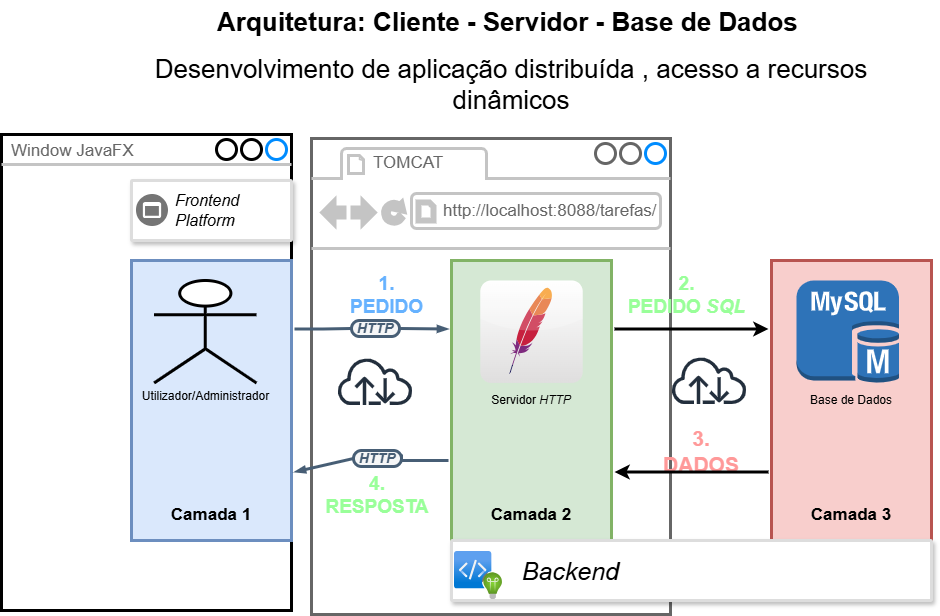
\includegraphics[scale=0.30]{figures/Diagrama-3-camada.drawio}
    \caption{Arquitetura distribuída de três camadas da aplicação \textit{Gestão de Tarefas}.}
    \label{fig:arquitetura}
\end{figure}

\noindent Como representado na Figura~\ref{fig:arquitetura}, o cliente \textit{JavaFX} não acede diretamente à base de dados, comunicando exclusivamente com o servidor \textit{Tomcat} através de pedidos \ac{http}.  O servidor, por sua vez, está na camada intermédia, com acesso à camada de dados, que comunica  com o \ac{sgbd} \textit{MySQL} através de \ac{jdbc}. 

\section{Modelo de Dados}
\label{sec:Ch3.3}

\noindent O modelo de dados da aplicação assenta em duas entidades principais: \textit{Utilizador} e \textit{Tarefa}, relacionadas entre si numa associação de um para muitos, já que um utilizador pode ser responsável por várias tarefas, mas cada tarefa pertence apenas a um utilizador. A Figura~\ref{fig:ermodel} apresenta o modelo relacional simplificado destas duas entidades.


\begin{figure}[htbp]
    \centering
    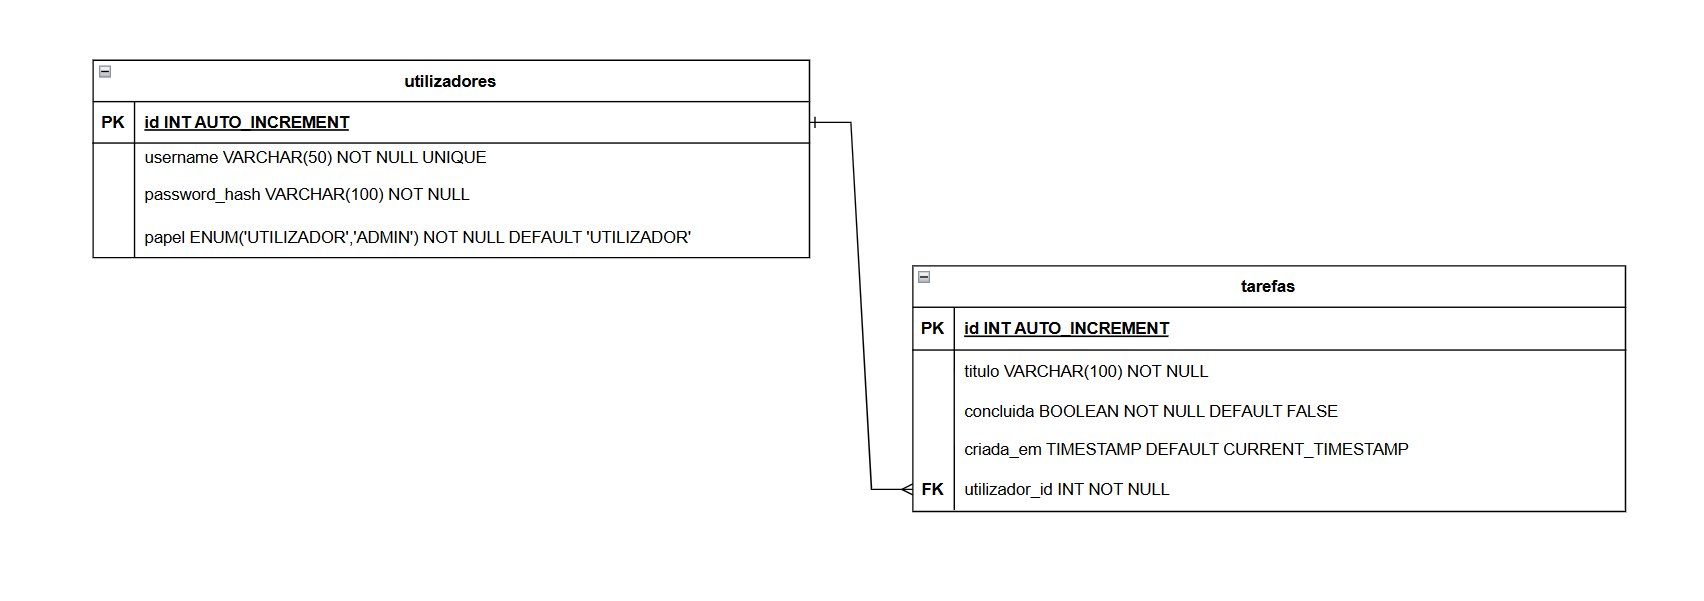
\includegraphics[scale=0.55]{figures/ModeloER.png}
  \caption{Modelo relacional simplificado das entidades \textit{Utilizador} e \textit{Tarefa}.}
	\label{fig:ermodel}
\end{figure}

\noindent Conforme ilustrado na Figura~\ref{fig:ermodel}, a entidade Utilizador armazena, entre outros campos, o atributo \code{perfil}, que distingue os registos do tipo Administrador dos registos do tipo \textit{Utilizador} comum, sendo este o campo consultado pelo \textit{back-end} para aplicar as regras de autorização descritas na Secção~\ref{sec:Ch3.2}. A entidade Tarefa inclui a chave estrangeira \code{idUtilizador}, que a associa ao seu responsável, bem como o campo \code{estado}, utilizado para representar o progresso da tarefa (por exemplo, por fazer, a fazer ou  concluída).

\section{Front-end}
\label{sec:Ch3.4}

\noindent O cliente gráfico  tem a estrutura correspondendo a cada uma a um ecrã da aplicação,  cada ecrã é associada a uma classe \textit{controller} \textit{JavaFX}, As respostas recebidas em \ac{json} são convertidas para objetos \textit{Java} antes de serem apresentadas.

\begin{itemize}
	\item \textbf{Autenticação:}~ecrã inicial onde o utilizador introduz as suas credenciais, submetidas ao \textit{endpoint} de autenticação do \textit{back-end};
	\item \textbf{Lista de Tarefas:}~apresenta, numa \code{TableView}, as tarefas do Utilizador autenticado ou, no caso do Administrador, a totalidade das tarefas registadas no sistema;
	\item \textbf{Formulário de Tarefa:}~permite a criação e a edição de uma tarefa, sendo reutilizado tanto para o Administrador como para o Utilizador;
	\item \textbf{Gestão de Utilizadores:}~ecrã exclusivo do Administrador, que lista os utilizadores registados e permite a sua criação e remoção.
\end{itemize}

A interface gráfica foi desenhada para adaptar as funcionalidades disponíveis ao perfil de acesso autenticado. Na Figura~\ref{fig:admin_view} apresenta-se a vista do utilizador com perfil de Administrador, destacando o acesso concorrente à gestão de tarefas e ao controlo de contas de utilizadores.


\begin{figure}[htbp]
    \centering
    \includegraphics[width=0.90\textwidth]{Gestao_tarefas-admin_view.png}
    \caption{Interface principal do sistema na perspetiva do perfil Administrador.}
    \label{fig:admin_view}
\end{figure}


Para além do desenho estético, a interface de autenticação contempla o tratamento imediato de erros de entrada de dados, alertando o utilizador em tempo real caso tente submeter o formulário sem preencher os campos obrigatórios (Figura~\ref{fig:login_validacao}).



\begin{figure}[htbp]
    \centering
    \includegraphics[width=0.45\textwidth]{Login.png}
    \caption{Ecrã de autenticação exibindo validação de campos obrigatórios.}
    \label{fig:login_validacao}
\end{figure}

A aplicação foi disponibilizada através de um servidor de aplicações Apache Tomcat, permitindo o acesso via navegador web. Na Figura~\ref{fig:web_admin_tarefas} é apresentada a interface Web acedida por uma conta de administrador, evidenciando as funcionalidades de gestão centralizada de todas as tarefas da plataforma, bem como o módulo de gestão e criação de novos utilizadores com diferentes níveis de privilégios.

\begin{figure}[htbp]
    \centering
    \includegraphics[width=0.90\textwidth]{tarefaslocalhost.png}
    \caption{Interface Web da aplicação em execução no Apache Tomcat (vista Administrador).}
    \label{fig:web_admin_tarefas}
\end{figure}

Em conformidade com as permissões atribuídas a cada conta, a interface Web adapta os elementos visíveis de acordo com o papel do utilizador autenticado. A Figura~\ref{fig:web_user_tarefas} ilustra a perspetiva de um utilizador comum (\texttt{eduardo}), demonstrando a restrição de acesso: este visualiza apenas as tarefas sob a sua responsabilidade e não dispõe de privilégios para apagar tarefas nem para aceder ao módulo de gestão de utilizadores.

\begin{figure}[htbp]
    \centering
    \includegraphics[width=0.50\textwidth]{eduardolocalhost.png}
    \caption{Interface Web no Apache Tomcat na perspetiva de um utilizador comum.}
    \label{fig:web_user_tarefas}
\end{figure}

\section{Back-end}
\label{sec:Ch3.5}

\noindent O \textit{back-end} é implementado como um conjunto de \textit{servlets} integrados dentro do \textit{Apache Tomcat}, organizados segundo o padrão \ac{dao} para o acesso aos dados, isolando as operações \ac{crud} sobre as entidades Utilizador e Tarefa da restante lógica de  \textit{front-end}. A Tabela~\ref{tab:endpoints} resume os principais \textit{endpoints} disponibilizados pela \ac{api} \ac{rest}.



\begin{table}[htb]
	\caption{\textit{Endpoints} da \ac{api} \ac{rest} do \textit{back-end}.}
	\label{tab:endpoints}
	\centering
	\begin{tabular}{l l l}
	\toprule
	\tabhead{Método} & \tabhead{Recurso} & \tabhead{Acesso} \\
	\midrule
		\code{POST} & \code{/auth/login} & Administrador \& Utilizador \\
		\code{GET} & \code{/tarefas} & Administrador (todas) \,/\, Utilizador (próprias) \\
		\code{POST} & \code{/tarefas} & Administrador \& Utilizador \\
		\code{PUT} & \code{/tarefas/\{id\}} & Administrador (todas) \,/\, Utilizador (próprias) \\
		\code{DELETE} & \code{/tarefas/\{id\}} & Administrador \\
		\code{GET} & \code{/utilizadores} & Administrador \\
		\code{POST} & \code{/utilizadores} & Administrador \\
		\code{DELETE} & \code{/utilizadores/\{id\}} & Administrador \\
	\bottomrule
	\end{tabular}
\end{table}

\noindent No âmbito da segurança e do princípio do menor privilégio, a ligação da base de dados é efetuada por uma conta de serviço dedicada, com acessos estritamente delimitados às tabelas necessárias (Figura~\ref{fig:db_utilizadores_privilegios}).

\begin{figure}[htbp]
    \centering
    \includegraphics[width=0.90\textwidth]{basedados_criar_utilizadores_privilegios.png}
    \caption{Configuração de privilégios de acesso e registos da tabela de utilizadores no MySQL Workbench.}
    \label{fig:db_utilizadores_privilegios}
\end{figure}

De forma a assegurar a modularidade e a clara separação de responsabilidades na camada de suporte ao servidor, o diretório de implementação organiza-se numa estrutura hierárquica bem delineada. Na Figura~\ref{fig:arvore_backend} apresenta-se a disposição dos diretórios principais.
\begin{figure}[htbp]
    \centering
    \includegraphics[width=0.75\textwidth]{tree_backend.png}
    \caption{Estrutura de pastas da aplicação evidenciando o módulo de suporte ao servidor Tomcat.}
    \label{fig:arvore_backend}
\end{figure}

\section{Sumário}
\label{sec:Ch3.6}

\noindent Neste capítulo descreveu-se a solução implementada para a aplicação \textit{Gestão de Tarefas}, assente numa arquitetura distribuída de três camadas que recorre ao \textit{JavaFX} na apresentação, ao \textit{Tomcat} na lógica de servidor e ao \textit{MySQL} na persistência de base de dados. As  camadas assim comunicam entre si por \ac{http}/\ac{json} e \ac{jdbc}, respetivamente.

%solução
%%%%%%%%%%%%%%%%%%%%%%%%%%%%%%%%%%%% Chapter Template

\chapter{Testes e Avaliação} 	% Main chapter titleTestes e Avaliação
\label{Chapter4} 		% For referencing the chapter elsewhere, 

%%%%%%%%%%%%%%%%%%%%%%%%%%%%%%%%%%%%


%%%%%%%%%%%%%%%%%%%%%%%%%%%%%%%%%%%%

\section{Funcionais}
\label{sec:Ch4.1}


\section{Desempenho}
\label{sec:Ch4.2}
% (volume de dados e latência por caso de uso e impacto da carga no caso maior latência)
\section{Usabilidade}
\label{sec:Ch4.3}


\section{Discussão }
\label{sec:Ch4.4}


\section{Sumário}
\label{sec:Ch4.5}







%testes e Avaliação
%%%%%%%%%%%%%%%%%%%%%%%%%%%%%%%%%%%% Chapter Template

\chapter{Conclusões} 	% Main chapter title
\label{Chapter5} 		% For referencing the chapter elsewhere,

%%%%%%%%%%%%%%%%%%%%%%%%%%%%%%%%%%%%


%%%%%%%%%%%%%%%%%%%%%%%%%%%%%%%%%%%%


\section{Sumário dos Resultados}
\label{sec:Ch5.1}


\section{Limitações}
\label{sec:Ch5.2}

\section{Desenvolvimento Futuro}
\label{sec:Ch5.3}



%Conclusão

%%%%%%%%%%%%%%%%%%%%%%%%%%%%%%%%%%%%%%%%%%%%%%%%%%%%%%%%%%%%%%%%%%%%%%%%%%%%%%%%%%%%%%%%%
% Print the bibliographic references using the ieeetr format from the 'sampleRefs.bib' file (root folder)

\printrefereces{sampleRefs}		% Change the 'sampleRefs' name to match your .bib file name,
								% a good option to make bib files is https://www.jabref.org/
%%%%%%%%%%%%%%%%%%%%%%%%%%%%%%%%%%%%%%%%%%%%%%%%%%%%%%%%%%%%%%%%%%%%%%%%%%%%%%%%%%%%%%%%%
\begin{appendices}
% Include the appendices of the dissertation as separate files from the 'chapters' folder

%% Appendix A

\chapter{Título do Anexo} % Main appendix title
\label{AppendixA} % For referencing this appendix elsewhere, use \ref{AppendixA}

%%%%%%%%%%%%%%%%%%%%%%%%%%%%%%%%%%%%%%%%%%%%%%%%%%%%%%%%%%%%%%%%%%%%%%%%%%%%%%%%%%
\section{Secção}

\lipsum[1]

%%%%%%%%%%%%%%%%%%%%%%%%%%%%%%%%%%%%%%%%%%%%%%%%%%%%%%%%%%%%%%%%%%%%%%%%%%%%%%%%%%
\section{Mais uma secção do Anexo~\ref{AppendixA}}

\lipsum[1]

	% Uncomment the lines as you write the appendices,
%\include{chapters/appendixB}	% or comment the lines if not used

\end{appendices}
%%%%%%%%%%%%%%%%%%%%%%%%%%%%%%%%%%%%%%%%%%%%%%%%%%%%%%%%%%%%%%%%%%%%%%%%%%%%%%%%%%%%%%%%%
\end{document}  
